\documentclass{lms}
\usepackage[utf8]{inputenc}
\usepackage[american]{babel}
\usepackage[T1]{fontenc}
\usepackage{amssymb,amsmath,amsfonts}
\usepackage{algorithmic}
\usepackage{algorithm}
\usepackage{tikz}
\usepackage{nicefrac}
\usepackage{hyperref}
\usepackage{unicode}
\usepackage{stmaryrd}
 
\newcommand{\todo}[1]{{\color{red}TODO: #1}}
\def\snote#1{\marginpar{{\color{blue}%
%   \rlap{\hskip 50pt \vrule height 1pt width 20pt}%
%   \leavevmode\kern 7pt \vbox{\hsize 56pt\kern -8pt
  \fontsize{7pt}{8pt}\selectfont #1\par}}}


%\theoremstyle{plain}
\newtheorem{thm}{Theorem}[section]
\newtheorem{lem}[thm]{Lemma}
\newtheorem{cor}[thm]{Corollary}
\newtheorem{prop}[thm]{Proposition}

\newnumbered{defi}{Definition}
\newnumbered{rem}{Remark}
\newnumbered{exe}{Example}
\newnumbered{prob}{Problem}

\def\mat#1{\begin{pmatrix}#1\end{pmatrix}}
\def\smat#1{{\def\arraystretch{.7}\mat{#1}}}
\def\pa#1{\left(#1\right)}
\def\bcro#1{\left\llbracket#1\right\rrbracket}
% pour les coûts des opérations M, F etc. (?)
\def\cout#1{\mathsf{#1}}

\newcommand{\F}{\mathbb{F}}
\newcommand{\Q}{\mathbb{Q}}
\newcommand{\C}{\mathbb{C}}
\newcommand{\tildO}{\tilde{O}}
\newcommand{\MM}{\cout{M}}
\newcommand{\FF}{\cout{F}}
\newcommand{\RR}{\cout{R}}
\DeclareMathOperator{\loglog}{loglog}

\def\algorithmicrequire{\textbf{Input:}}
\def\algorithmicensure{\textbf{Output:}}

\makeatletter
\def\full@line{8pt}
\def\doublefull@line{12pt}
% \def\@nprf{% nprf environment modified OT 12/11/02
%   \list{}{\topsep 8pt \leftmargin 0pt
%   \itemindent\parindent \labelsep .5em 
%   \listparindent\parindent
%   \settowidth\labelwidth{{\normalfont\rmfamily(iii)}}}%
%   \item{\normalfont\itshape\proofname.}\advance\itemindent\labelsep%
%   \advance\itemindent\labelwidth%
%   \hskip 1em\normalfont\rmfamily\ignorespaces}
\makeatother


% Colors after XKCD color name survey
\definecolor{purple}{rgb}{.49,.11,.61}
\definecolor{green}{rgb}{.08,.69,.10}
\definecolor{blue}{rgb}{.01,.26,.87}
\definecolor{pink}{rgb}{1,.5,.75}
\definecolor{brown}{rgb}{.39,.21,.00}
\definecolor{red}{rgb}{.89,0,0}
\definecolor{lightblue}{rgb}{.58,.81,.98} 
\definecolor{teal}{rgb}{0,.57,.52}
\definecolor{orange}{rgb}{.97,.45,.02}
\definecolor{lightgreen}{rgb}{.53,.99,.01}
\definecolor{magenta}{rgb}{.76,0,.47}
\hypersetup{colorlinks,linkcolor={red!70!black},
  citecolor={green!70!black},urlcolor={blue!70!black}}

\title[Explicit isogenies in any characteristic]{Explicit isogenies in quadratic time in any characteristic}
\author{Cyril Hugounenq}

\classno{11Y40 (primary), 11G20, 14H52 (secondary)}

\extraline{This work was partially supported by the
  \href{http://www.digiteo.fr/}{DIGITEO} grant 2013-0531D (ARGC).}

\begin{document}
\maketitle

\begin{abstract}
The problem we will consider here is the computation of an isogeny between two elliptics curves with the knowledge of the domain and the codomain of the isogeny and it's degree $r$. Couveignes's algorithm is an algorithm which solves this problem in $O(r^2)$ operations using the $p$-torsion. We want to extend the method used by Couveignes  We try to adapt his method here to the case of the $2$ torsion and more generally to the $\ell$ torsion, thus we propose an alternative for medium characteristic with this algorithm.
\end{abstract}

% \section*{Proposed notation}

% This section is for internal reference only: erase after the paper has
% stabilized.

% \begin{itemize}
% \item $\mathbb{F}_q$ is the field we are working on
% \item $\ell$ is for the $\ell$ torsion we are working on
% \item $r$ is the degree of the isogeny we want to compute
% \item $k$ is the integer such that $\ell^{2k}>4r+1$
% \item we thus work with a tower which has for top level $F_{q^{\ell^k}}$
% \item $E$ is for ordinary elliptic curves defined over the finite field $\mathbb{F}_q$
% \item $\mathcal{O}$ (resp. $\mathcal{O}_x$) is the notation for the endomorphism ring associated (up to isomorphism) to $E$ (resp. $E_x$)
% \item $K$ is the notation for the imaginary quadratic field in which $\mathcal{O}$ is defined
% \item $d_K$ is the negative integer such that $K=\mathbb{Z}[d_K]$  
% \end{itemize}

%%%%%%%%%%%%%%%

\section{Introduction}
\label{sec:introduction}

Isogenies are non-zero morphisms of elliptic curves, that is,
non-constant rational maps preserving the point at infinity. They are
also algebraic group morphisms. Isogeny computations play a central
role in the algorithmic theory of elliptic curves. They are notably
used to speed up Schoof's point counting
algorithm\cite{schoof85,atkin88,elkies92,schoof95,elkies98}. They are
also widely applied in cryptography, where they are used to speed up
point multiplication~\cite{gallant+lambert+vanstone01,birkner+sica11},
to perform cryptanalysis~\cite{mauer+menezes+teske01}, and to
construct new
cryptosystems~\cite{teske06,charles+lauter+goren09,Stol,defeo+jao+plut12,jao+soukharev2014-signatures}.

The \emph{degree} of an isogeny is its degree as a rational map. If an
isogeny has degree $r$, we call it an $r$-isogeny, and we say that two
elliptic curves are $r$-isogenous if there exists an $r$-isogeny
relating them. Accordingly, we say that two field elements $j$ and
$j'$ are $r$-isogenous if there exist $r$-isogenous elliptic curves
$E$ and $E'$ such that $j(E)=j$ and $j(E')=j'$. The
\emph{explicit isogeny} problem has many incarnations. In this paper,
we are interested in the variant defined below.

\begin{prob}[(Explicit isogeny problem)] \label{prob:isogeny-problem}
  Given two $j$-invariants $j$ and $j'$, and a positive integer
  $r$, determine if they are $r$-isogenous. In that case, compute
  curves $E$, $E'$ with $j(E)=j$ and $j(E')=j'$, and the
  kernel of an $r$-isogeny $ψ:E\to E'$.
\end{prob}

Once the kernel of the isogeny is computed, the rational maps
associated to it can be computed in optimal time using Velu's
formulas~\cite{velu71}.

This paper focuses on the explicit isogeny problem for \emph{ordinary}
elliptic curves over finite fields. A famous theorem by Tate states
that two curves are isogenous over a finite field if and only if they
have the same cardinality over that field. The explicit isogeny
problem stated here appears naturally in the Schoof-Elkies-Atkin point
count algorithm (SEA). There, $E$ is the curve of which we want to
compute the cardinality, and $E'$ is an $r$-isogenous curve, with $r$
a prime of size approximately $\log\#E$. For this reason, the explicit
isogeny problem is customarily solved without prior knowledge of the
cardinality of $E$. We will abide by this convention here.

A good measure of the computational difficulty of the problem is given
by the isogeny degree $r$. Indeed the output is represented by
$O(r)$ base field elements, hence an asymptotically optimal algorithm
would solve the problem using $O(r)$ field operations. Many algorithms
have been suggested over the years to solve the explicit isogeny
problem. Early algorithms were due to Atkin~\cite{atkin91} and
Charlap, Coley and
Robbins~\cite{charlap1991enumeration}. Elkies'~\cite{elkies92,elkies98,Bostan}
was the first algorithm targeted to finite fields (of large enough
characteristic). Assuming $r$ is prime, its complexity is dominated by
the computation of the modular polynomial $\Phi_r$, which is an object
of (binary) size $O(r^3\log r)$. Later Bröker, Lauter and
Sutherland~\cite{sutherland10:modpol} optimized the modular polynomial
computation in the context of the SEA
algorithm. Finally Lercier and Sirvent\cite{lercier+sirvent08,1602.00244}
generalized Elkies' algorithm to work in any characteristic. Despite
these advances, the overall cost of Elkies' algorithm and its
variants is still at least cubic in $r$.

Another line of work to solve the explicit isogeny problem was
initiated by Couveignes~\cite{couveignes94,couveignes96,couveignes00},
and later improved by De Feo and Schost~\cite{df10,df+schost12}. These
algorithms use an interpolation approach combined with ad-hoc
constructions for towers of finite fields of characteristic $p$. Their
complexity is quasi-quadratic in $r$, but exponential in $\log p$,
hence they are only practical for very small characteristic.

In this paper we present a variant of Couveignes' algorithm with
complexity polynomial in $\log p$ and quasi-quadratic in $r$. Together
with the Lercier-Sirvent algorithm, they are the only polynomial-time
isogeny computation algorithms working in any characteristic, hence
they are especially relevant for counting points in \emph{medium}
characteristic (i.e., counting points over $\F_{p^n}$, when
$n\gg p/\log p$).

Note that, although Couveignes-type algorithms do not make use of the
modular polynomial $\Phi_r$, its computation is still necessary in the
context of the SEA algorithm. Thus our new algorithm does not improve
the state of the art on point counting \todo{but maybe benchmarks are
  going to show that, at least in practice, we sometimes beat
  Lercier-Sirvent?}. It gives, however, an effective algorithm for
solving the explicit isogeny problem, with potential applications in
other contexts, e.g., cryptography.

\subsection{Notations}

Throughout this paper: $r$~is a positive integer, $p$~an odd prime,
$q$~a power of $p$, and $\mathbb F_q$ is the finite field with
$q$~elements. $E$ ~is an ordinary elliptic curve over~$\mathbb F_q$,
its group of $n$-torsion points is denoted by~$E[n]$, its
$q$-Frobenius automorphism by~$π$.  The endomorphism ring of $E$ is
denoted by~$\mathcal O$, with~$K = \mathcal O ⊗ ℚ$ the corresponding
number field, $\mathcal O_K$ is its maximal order, and $d_K$~the
discriminant of~$\mathcal O_K$.  For a prime~$ℓ$ different from~$p$
and not dividing~$r$, we denote by~$T_ℓ(E) = \varprojlim E[ℓ^n]$ the
$ℓ$-adic Tate module~\cite[III.7]{Sil}, which is free of rank~two
over~$ℤ_ℓ$.  The factorization of the characteristic polynomial of~$π$
in~$ℤ_ℓ$ is determined by the Kronecker symbol~$(d_K/ℓ)$.  If
$(d_K/ℓ) = +1$ then we also define $λ,μ$ as the eigenvalues of~$π$
in~$ℤ_ℓ$ and write~$h = v_ℓ(λ - μ)$, where $v_ℓ$ is the $ℓ$-adic
valuation.

We measure all computational complexities in terms of operations in
$\mathbb{F}_q$, we use the \emph{big-Oh} notation $O()$ to express
asymptotic complexities, and the notation $\tildO()$ to neglect
polylogarithmic factors.  We let $\MM(n)$ be a function such that
polynomials in $\F_q[X]$ of degree less than $n$ can be multiplied
using $\MM(n)$ operations in $\F_q$, under the assumptions
of~\cite[Ch.~8.3]{vzGG}. Using FFT multiplication, one can take
$\MM(n)∈ O(n\log n\loglog n)$.

The algorithms presented next operate on elements defined in finite
extensions of $\F_q$. Specifically, we define a \emph{tower} of finite
fields $\F_q=F₀⊂F₁⊂\cdots⊂F_k$ with $[F₁:F₀]$ dividing $ℓ-1$, and
$[F_{i+1}:F_i]∈\{1,ℓ\}$ for any $i>0$. For $ℓ=2$, we build upon the
work of Doliskani and Schost~\cite{DoSc12}, while for general $ℓ$ we
use towers of Kummer extensions as described
in~\cite[\S~2]{DeDoSc13}. Using these constructions, we are able to
perform the following operations:
\begin{itemize}
\item basic arithmetic operations (addition, multiplication) in $F_i$,
  using $O(\MM(ℓ^i))$ operations;
\item inversion in $F_i$ using $O(i\MM(ℓ^i)\logℓ)$
  operations\footnote{When $ℓ=2$, a factor of $i$ can be saved
    here~\cite{DoSc12}, but we will disregard this optimization for
    simplicity.};
\item mapping elements from $F_{i-1}$ to $F_i$ and \emph{vice versa}
  at no arithmetic cost;
\item multiplication and Euclidean division of polynomials of degree
  at most $d$ in $F_i[x]$ using $O(\MM(dℓ^i))$ operations.
\end{itemize}

Finally, we introduce the notations $\FF(i,j)$ for the cost of
computing a $q^{ℓ^j}$-th power in $F_i$, and $\RR(i)$ for the cost of
finding a root of a polynomial of degree $ℓ$ in $F_i[x]$. When
$\ell=2$, Doliskani and Schost show that $\FF(i,j)=O(ℓ^i+\log q)$, and
$\RR(i)=O(\MM(ℓ^i)\log(ℓ^iq))$. For general $ℓ$, we have
$F(i,j)=O(ℓ^{i+j}\log q)$ using a naive algorithm, and
$\RR(i)=O(ℓ^i\MM(ℓ^{i+1})\logℓ\log(ℓq))$ using the variant of the
Cantor-Zassenhaus algorithm described in \cite[\S~14.5]{vzGG} \todo{we
  could use Kalto-Shoup here}.


\subsection{Couveignes' algorithm}
\label{sec:couv-algor}

Couveignes' isogeny algorithm takes as input two \emph{ordinary}
elliptic curves $E$ and $E'$, and a positive integer $r$ not
divisible by $p$, and returns, if it exists, the kernel of an
$r$-isogeny $ψ:E\to E'$. It is based on the observation that the
isogeny $ψ$ must put $E[p^k]$ in bijection with $E'[p^k]$, in a way
that is compatible with their group structure. It proceeds in three
steps:
\begin{enumerate}
\item\label{alg:orig-couveignes:tower} Compute generators $P,P'$ of
  $E[p^k]$ and $E'[p^k]$ respectively, for $k$ large enough;
\item\label{alg:orig-couveignes:interp} Compute the interpolation
  polynomial $\mathcal{A}$ \todo{(verify that notation is consistent
    with Sec.5)} sending $x(P)$ to $x(P')$, and the abscissas of
  their scalar multiples accordingly;
\item\label{alg:orig-couveignes:rational} Deduce a rational fraction
  congruent to $\mathcal{A}$ modulo $E[p^k]$, and verify that it
  defines an isogeny of degree $r$. If it does, return it, otherwise
  replace $P'$ with a scalar multiple of itself and go back to
  Step~\ref{alg:orig-couveignes:interp}.
\end{enumerate}

For this algorithm to succeed, enough interpolation points are
required. Given that the isogeny $ψ$ is defined by a rational fraction
of degree $(r,r-1)$, it is necessary that $p^k∈O(r)$. However, most of
the time, those points are not going to be defined in the base field
$\F_q$, thus Couveignes' algorithm must be based on efficient
algorithms to construct and compute in towers of extensions of finite
fields. Indeed, Couveignes and his successors go at great length in
studying the arithmetic of \emph{Artin-Schreier
  towers}~\cite{couveignes00,df+schost12}, and the adaptation of the
fast interpolation algorithm to that setting~\cite{df10}.  Using these
highly specialized constructions,
Steps~\ref{alg:orig-couveignes:tower}
and~\ref{alg:orig-couveignes:interp} are both executed in quasi-linear
time $\tildO(p^{k+O(1)})=\tildO(rp^{O(1)})$. However the last step
only succeeds for one pair of torsion points $P,P'$, in general, thus
$O(r)$ trials are expected on average.

Hence, the overall complexity of Couveignes' algorithm is
$\tildO(r²p^{O(1)})$, i.e., quadratic in $r^2$, but exponential in
$\log p$. Although the exponent of $\log p$ is relatively small, Couveignes
algorithm quickly becomes impractical as $p$ grows. In this paper we
introduce a variant of Couveignes' algorithm with the same quadratic
complexity in $r$, and \textbf{no exponential dependency in $\log p$}.

The bottom line of our algorithm is elementary: replace $E[p^k]$ in
the algorithm with $E'[ℓ^k]$, for some small prime $ℓ$. However a
naive application of this idea fails to yield a quadratic-time
algorithm. Indeed, in the worst case one has $ℓ^{2k}∈O(r)$, with
$E[ℓ^k]≃(ℤ/ℓ^kℤ)²$. Hence, two generators $P,Q$ of $E[ℓ^k]$ must
be mapped onto two generators of $E'[ℓ^k]$. This can be done in
$O(ℓ^{4k})$ possible ways \todo{double check this}, thus yielding an
algorithm of complexity $\tildO(ℓ^{6k})=\tildO(r³)$.

To avoid this pitfall, we must carefully study the structure of
$E[ℓ^k]$, and its relationship with the Frobenius endomorphism $π$,
which we do in the next section. With that knowledge, we will be able
to put some restrictions on the generators $P,Q$, thus limiting the
number of trials to $O(ℓ^{2k})$, as explained in
Section~\ref{sec:acti-frob-endm}.  In Section~\ref{sec:interpolation}
we present an interpolation algorithm adapted to the setting of
$ℓ$-adic towers, and in Section~\ref{sec:complete-algorithm} we put
all steps together and analyze the full algorithm. Finally in
Section~\ref{sec:implem} we discuss our implementation and the
performances of the algorithm.


%%%%%%%%%%%%%%%

\section{Isogeny volcanoes}
\label{sec:isogeny-volcanoes}

\todo{Notions de base sur les isogenies et les volcans.}

For an extensive introduction to isogeny volcanoes we address the
reader to~\cite{sutherland2013isogeny}.

\subsection{The graph of $ℓ$-isogenies}

We write~{$ℓ$-isogeny} for an isogeny of degree~$ℓ$.
We recall without their proof two results about
$ℓ$-isogenies between ordinary elliptic curves.

\begin{prop}[{\cite[Proposition~21]{Kohel}}] \label{prop:isogeny-asc-desc}
Let~$ϕ: E → E'$ be an $ℓ$-isogeny between ordinary elliptic curves
and~$\mathcal O, \mathcal O'$ be their endomorphism rings.
Then one of the three following cases is true:
\begin{enumerate}
\item $[\mathcal O':\mathcal O] = ℓ$,
in which case we call $ϕ$ \emph{ascending};
\item $[\mathcal O:\mathcal O'] = ℓ$,
in which case we call $ϕ$ \emph{descending};
\item $\mathcal O' = \mathcal O$,
in which case we call $ϕ$ \emph{horizontal}.
\end{enumerate}
\end{prop}
\begin{prop}[{\cite[Proposition~23]{Kohel}; \cite[Lemma~6]{sutherland2013isogeny}}] \label{prop:isogeny-count}
Let~$E$ be an ordinary elliptic curve with endomorphism ring~$\mathcal O$.
\begin{enumerate}
\item if $\mathcal O$~is maximal then
there are $(d_K/ℓ)+1$~horizontal $ℓ$-isogenies from~$E$
(and no ascending $ℓ$-isogenies).
\item if $\mathcal O$~is not maximal then
there are no horizontal $ℓ$-isogenies from~$E$,
and one ascending $ℓ$-isogeny.
\end{enumerate}
\end{prop}

A \emph{volcano of $ℓ$-isogenies} is a connected component
of the graph of $ℓ$-isogenies between curves defined on~$\mathbb F_q$.
The \emph{crater} is the subgraph corresponding to curves
having the maximal endomorphism ring~$\mathcal O_K$.
The shape of the crater is given by the Kronecker symbol~$(d_K/ℓ)$,
as per Proposition~\ref{prop:isogeny-count}.
For any~$n ≥ 0$, a $ℓ^n$-isogeny is \emph{horizontal}
if it is the composite of $n$~horizontal $ℓ$-isogenies.
We say that a point~$P ∈ E[ℓ^n]$ is \emph{horizontal}
if the isogeny~$ϕ_P$ with kernel~$P$ is horizontal.
The \emph{depth} of a curve is its distance from the crater.
It is also the $ℓ$-adic valuation of the conductor
of~$\mathcal O = \mathrm{End}(E)$.

		\begin{figure}[h]
		\begin{center}
		
        \begin{tikzpicture}[scale=0.3]
        \coordinate (A) at (0,0);
		\coordinate (B) at (230:5);
		\coordinate (C) at (270:4);
		\coordinate (D) at (310:5);
		\draw (A) node{$\bullet$};
		\draw (B) node{$\bullet$};
		\draw (C) node{$\bullet$};
		\draw (D) node{$\bullet$};
		\node at (0,-6.7) {$(d_K/ℓ) = -1$};
		\draw (A)--(B);
		\draw (A)--(C);
		\draw (A)--(D);
		
		\begin{scope}[xshift=9cm]
		\coordinate (A) at (0,0);
		\coordinate (B) at (5.5,0);
		\coordinate (C) at (240:4.2);
		\coordinate (D) at (300:4.2);
		\draw (A) node{$\bullet$};
		\draw (B) node{$\bullet$};
		\draw (C) node{$\bullet$};
		\draw (D) node{$\bullet$};
		\node at (2.8,-6.7) {$(d_K/ℓ) = 0$};
		\draw (A)--(B);
		\draw (A)--(C);
		\draw (A)--(D);
		\end{scope}
		
		\begin{scope}[xshift=14.5cm]
		\coordinate (A) at (0,0);
		\coordinate (C) at (240:4.2);
		\coordinate (D) at (300:4.2);
		\draw (A) node{$\bullet$};
		\draw (C) node{$\bullet$};
		\draw (D) node{$\bullet$};
		\draw (A)--(C);
		\draw (A)--(D);
		\end{scope}
		
		\begin{scope}[xshift=23cm]
		\node (A) at (-3,0) {$\bullet$};
		\node (B) at (3,0) {$\bullet$};
		\node (C) at (270:1.2) {$\bullet$};
		\node (D) at (90:1.5) {};
		\node at (0,-6.7) {$(d_K/ℓ) = +1$};
		%\draw[-] (A.center) to[bend right=25] (C.center);
		\draw[-,dashed] (A.center) to[bend left=40] (B.center);
		%\draw[-] (B.center) to[bend left=25] (C.center);
		%\draw[-,dashed] (B.center) to[bend right] (D.center);
		\draw[-] (A.center) to[bend right=40] (B.center);
			\begin{scope}[xshift=-3cm]
			\coordinate (A) at (0,0);
			\coordinate (C) at (270:4.2);
			\draw (A) node{$\bullet$};
			\draw (C) node{$\bullet$};
			\draw (A)--(C);
			\end{scope}
			\begin{scope}[xshift=3cm]
			\coordinate (A) at (0,0);
			\coordinate (C) at (270:4.2);
			\draw (A) node{$\bullet$};
			\draw (C) node{$\bullet$};
			\draw (A)--(C);
			\end{scope}
			\begin{scope}[yshift=-1.2cm]
			\coordinate (A) at (0,0);
			\coordinate (C) at (270:4.2);
			\draw (A) node{$\bullet$};
			\draw (C) node{$\bullet$};
			\draw (A)--(C);
			\end{scope}
		\end{scope}
		\end{tikzpicture}
		%\end{center}
		\caption{The three shapes of volcanoes of $2$-isogenies }
		
		\end{center} 
		\end{figure}
\subsection{The Frobenius and the volcano}

During the rest of this paper we consider only a volcano with a cyclic crater
(i.e. we assume $\left( \frac{d_K}{\ell} \right) =1$).
This implies that the Frobenius automorphism on~$T_ℓ(E)$,
which we write~$π|T_ℓ(E)$, has two distinct eigenvalues~$λ ≠ μ$.

\begin{prop}\label{prop:matrice-frobenius}
Let~$E$ be an ordinary elliptic curve with Frobenius endomorphism~$π$.
Assume that the characteristic polynomial of~$π$
has two distinct roots~$λ, μ$ in~$ℤ_ℓ$,
so that the $ℓ$-isogeny volcano has a cyclic crater.
Then there exists a unique $a ∈ \llbracket 0, ℓ^h - 1 \rrbracket$
such that $π|T_ℓ(E)$~is conjugated, over~$ℤ_ℓ$,
to the matrix $\smat{λ & a\\ 0 & μ}$.
% where $a ∈ ℤ$, $0 ≤ a ≤ ℓ^{h} - 1$,
Moreover $a = 0$ if~$E$ lies on the crater,
and else $h - v_{ℓ}(a)$~is the depth of~$E$ in the volcano.
\end{prop}
\begin{proof}
Since the characteristic polynomial of~$π$ splits over~$ℤ_ℓ$,
the matrix of~$π|T_ℓ(E)$ is trigonalizable.
Conjugating the matrix $\smat{λ & a\\0 & μ}$
by~$\smat{1 & b\\0 & 1}$ replaces~$a$ by~$a + b (λ - μ)$.
Finally, by Tate's theorem~\cite[Isogeny theorem 7.7 (a)]{Sil},
$\mathcal O ⊗ ℤ_ℓ$~is isomorphic to the order in~$ℤ_ℓ[π_ℓ]$
of matrices with integer coefficients,
which is generated by the identity and~$ℓ^{-v_ℓ(a)} π_ℓ$.
\end{proof}

A basis of~$E[ℓ^n]$ is \emph{diagonal} if $π$~is diagonal in this basis;
it is \emph{horizontal} if both basis points generate the kernel of
horizontal $ℓ^n$-isogenies.
The link between horizontal and diagonal bases is given below.
% The $ℓ+1$ isogenies of degree~$ℓ$ are parametered by $\mathbb P^1(ℤ/ℓZ)$.
% Namely, let~$(P, Q)$ be a basis of~$E[ℓ]$;
% we define~$ε_i$ as the isogeny with kernel~$P + i Q$ if~$i ∈ ℤ/ℓℤ$,
% and~$Q$ if~$i = ∞$.
% The action of these isogenies on the Tate modules is given by
% $T_ℓ(ε_i) = \smat{ℓ & i\\0&1}$ and~$T_ℓ(ε_∞) = \smat{1&0\\0&ℓ}$.
% In particular, the two eigenvalues of~$π$ correspond canonically to
% the two horizontal $ℓ$-isogenies.
% If~$λ ≡ μ \pmod{ℓ}$ then $π|E[ℓ]$ is a scalar matrix,
% and does not contain enough information
% to identify these directions.
% To make this identification precise,
% we need to consider the $ℓ^k$-torsion for~$k ≥ h+1$.
% The following proposition is then a direct consequence
% of Proposition~\ref{prop:matrice-frobenius}.

\begin{prop} \label{prop:diagonal-horizontal}
Let~$E$ be a curve lying on the crater and~$P$ be a point of~$E[ℓ^n]$.
Then $ℓ^h P$~is horizontal if, and only if, $P$~is an eigenvector for~$π$.
(If $π(P) = λ P$ then we say that $ℓ^h P$~has the direction~$λ$).
\end{prop}
\begin{proof}
Fix a basis~$(R, S)$ of~$E[ℓ^n]$ that diagonalizes~$π$.
We can write $P = a R + b S$; w.l.o.g. we may assume $b=1$.
Let~$E'$ be the image curve of~$ϕ_{ℓ^h P}$.
Then $π|T_ℓ(E')$ has the matrix~$\smat{λ& ℓ^{h-n} a (μ-λ)\\ 0&μ}$.
This matrix is diagonalizable only if~$v_{ℓ}(a) ≥ n - h$.
On the other hand, we can compute~$(π - μ) P = a (λ - μ) R$,
so that $P$~is an eigenvector on the same condition~$v_{ℓ}(a) ≥ n-h$.
\end{proof}

While horizontal bases are our main interest,
diagonal bases are easier to compute in practice.
Algorithms computing both kind of bases
are given in Section~\ref{sec:acti-frob-endm}.
The main tool for this is the next proposition:
given a horizontal point of order~$ℓ^n$,
it allows us to compute a horizontal point of order~$ℓ^{n+1}$.

\begin{prop}\label{prop:push-horizontal}
Let~$ψ: E → E'$ be a horizontal $ℓ$-isogeny with direction~$λ$.
For any point~$Q$ such that~$ℓ · Q$ is horizontal with direction~$μ$,
$ψ(Q)$ is horizontal with direction~$μ$.
\end{prop}
\begin{proof}
Let~$Q' = ψ(Q)$ and~$\widehat{ψ}$ be the isogeny dual to~$ψ$.
Since both $\widehat{ψ}$~and~$\widehat{ψ}(Q') = ℓ Q$ are horizontal
with direction~$μ$, $Q'$~is also horizontal.
\end{proof}
\medbreak

As another simple consequence of Proposition~\ref{prop:matrice-frobenius},
we may bound the degree of extensions containing points of $ℓ^n$-torsion.
\begin{prop}\label{prop:degree-l-torsion}
For any~$n$, let~$d(n)$ be the smallest integer
such that all the points of~$E[ℓ^n]$ are rational over~$\mathbb F_{q^{d(n)}}$.
Then:
\begin{enumerate}
\item $d(1)$ divides~$(ℓ-1)$.
\item There exists a constant~$c ≥ 0$ such that, for all~$n ≥ c$,
$d(n) = d(1) · ℓ^{n-c}$.
\end{enumerate}
\end{prop}
\begin{proof}
The degree~$d(n)$ is exactly the order of the matrix~$π|E[ℓ^n]$.
It is therefore the least common multiple of the multiplicative orders
of~$λ, μ$ modulo~$ℓ^n$.
We conclude using the multiplicative structure of~$(ℤ/ℓ^n ℤ)^×$.
% To conclude we use the canonical decomposition:
% $(ℤ/ℓ^nℤ)^× = (ℤ/ℓℤ)^× × (ℤ/ℓ^{n-1} ℤ)$ for~$ℓ ≠ 2$,
% and $(ℤ/2^{n} ℤ)^× = (ℤ/4ℤ)^× × (ℤ/2^{n-2} ℤ)$ for~$ℓ = 2$.
\end{proof}


\begin{prop}\label{prop:isogenie-premiere}
Let~$ψ: E → E'$ be an isogeny of degree~$r$ prime to~$ℓ$.
\begin{enumerate}
\item The curves~$E$ and~$E'$ have the same depth
in their $ℓ$-isogeny volcanoes.
\item For any point~$P ∈ E[ℓ^n]$,
the isogenies with kernel $P$ and~$ψ(P)$ have the same type
(ascending, descending, or horizontal with the same direction).
\item If $P ∈ E[ℓ]$ and $P' ∈ E'[ℓ]$ are both ascending,
or both horizontal with the same direction,
then $E/P$ and~$E'/P'$ are again $r$-isogenous.
\end{enumerate}
\end{prop}
\begin{proof}
Points~(i) and~(ii) are consequences of Proposition~\ref{prop:matrice-frobenius}
and of the fact that $ψ$, being rational and of degree prime to~$ℓ$,
induces an isomorphism between the Tate modules of~$E$ and~$E'$,
commuting to the Frobenius endomorphisms.
For point~(iii), we just note that
since there exists a unique point of order~$ℓ$
either ascending or horizontal with a given direction,
we must have~$P' = ψ(P)$.
\end{proof}

% \begin{proof}
% $E_{\lambda_1}=\{P \in E[\ell],  \pi(\frac{P}{\ell^h})=\lambda_1\frac{P}{\ell^h}\}$, $E_{\lambda_2}=\{P \in E[\ell],  \pi(\frac{P}{\ell^h})=\lambda_2\frac{P}{\ell^h}\}$ and consider $\phi_1$(resp. $\phi_2$) the $\ell$isogeny generated by $E_{\lambda_1}$ (resp. $E_{\lambda_2}$).
% since we have a cyclic crater $\left( \frac{d_K}{\ell} \right)=1$ then (by Proposition 5.11 of \cite{Cox89} )  $\ell \mathcal{O}_K=\mathfrak{l}_1\mathfrak{l}_2$ with $Gal(K/\mathbb{Q})$ such as $\mathfrak{l}_1'=\mathfrak{l}_2$ (by theorem 5.9 of \cite{Cox89}).
% On veut faire pareil en disant que $E_{\lambda_1}=(\ell, \frac{\pi - \lambda_1}{\ell^h})$ idem pour $\lambda_2$, tel que $\ell=(\ell, \frac{\pi - \lambda_1}{\ell^h})(\ell, \frac{\pi - \lambda_2}{\ell^h})$, par un résultat dans Advanced Topics de Silverman, il ne reste plus qu'à prouver que cette décomposition de l'idéal $\ell$ est une décomposition en idéaux premiers. 
% %%%%Ancienne preuve avec de très nombreux défauts
% %We denote by $E_{\lambda_1}=\{P \in E[\ell^{h+1}], \ell^{h}P \neq 0, \pi(P)=\lambda_1P\}$, $E_{\lambda_2}=\{P \in E[\ell^{h+1}], \ell^{h}P \neq 0, \pi(P)=\lambda_2P\}$ and consider $\phi_1$(resp. $\phi_2$) the $\ell$isogeny generated by $E_{\lambda_1}$ (resp. $E_{\lambda_2}$). This isogeny is unique since those eigenspace are of dimension $1$. % on pourrait se passer de cette dernière phrase... 
% %We remind that we have the endomorphism ring of $E$: $\mathcal{O} \subset \mathcal{O}_K $ and $[\mathcal{O}:\mathcal{O}_K] =1$, since we have a cyclic crater $\left( \frac{d_K}{\ell} \right)=1$ then (by Proposition 5.11 of \cite{Cox89} )  $\ell \mathcal{O}_K=\mathfrak{l}_1\mathfrak{l}_2\mathcal{O}_K$ with $Gal(K/\mathbb{Q})$ such as $\mathfrak{l}_1'=\mathfrak{l}_2$ (by theorem 5.9 of \cite{Cox89}). Since $E_{\lambda_1}$ and $E_{\lambda_2}$ are also conjugated with $Gal(K/\mathbb{Q})$ we can associate to the isogeny $\phi_1$ (resp. $\phi_2$)  the integral ideal $\mathfrak{l}_1\mathcal{O}_K$ (resp. $\mathfrak{l}_2\mathcal{O}_K$) and the endomorphism ring $\mathfrak{l}_1^{-1}\mathcal{O}_K$ (resp. $\mathfrak{l}_2^{-1}\mathcal{O}_K$) to their codomain. Since we got $\mathfrak{l}_1\mathfrak{l}_2=\ell$ then $\mathfrak{l}_1^{-1}=\left( \frac{\mathfrak{l}_2}{\ell} \right)$ therefore $[\mathcal{O}_K:\left( \frac{\mathfrak{l}_2}{\ell} \right)\mathcal{O}_K]\wedge \ell =1$. The others isogenies are those associated to the integral ideals $a  \mathfrak{l}_1 + \mathfrak{l}_2$ with $a \wedge \ell =1$ and to the groups which are generated by a linear combination of points of $E_{\lambda_1}$ and $E_{\lambda_2}$
% \end{proof}
% 


%%%%%%%%%%%%%%%


\section{Computing the action of the Frobenius endomorphism}
\label{sec:acti-frob-endm}

\subsection{Computation of a diagonal basis}
\label{ss:diagonal}

In this part, given an elliptic curve~$E$ belonging to the crater
of an $ℓ$-isogeny volcano, we explicitly diagonalize the Frobenius endomorphism
in~$E[ℓ^k]$, where $k ≥ h+1$,
in order to identify the directions of the two horizontal $ℓ$-isogenies.
By Proposition~\ref{prop:degree-l-torsion},
replacing~$\mathbb F_q$ with an extension of degree up to~$ℓ - 1$,
we may assume that all the points of~$E[ℓ]$ are rational over~$\mathbb F_q$;
then all the points of~$E[ℓ^k]$ are rational over~$\mathbb F_{q^{ℓ^k}}$.
Therefore, all our algorithms work in~$\mathbb F_{q^{ℓ^k}}$.
All the complexities are given as a number of
operations in the base field~$\mathbb F_q$.
\todo{référer à la partie qui explique les complexités du calcul dans les
extensions, quand elle sera écrite}

%We first give an algorithm computing a preimage of a rational point of~$E$
%by multiplication by~$ℓ$, when such a preimage exists.
%For convenience we assume that~$E[\ell]$ is rational over~$\mathbb{F}_q$.
%If this is not the case, we may always replace~$q$ by~$q^{\ell-1}$.


% We restrict ourselves to the case where $E[\ell] \subset E(\mathbb{F}_q)$, because we just have to work in $\mathbb{F}_{q^{\ell-1}}$ to have this hypothesis true.
% 
% From this point we study the $\ell$ torsion points that are eigenvector for the Frobenius, thus we work in this section only with curves that are on the cyclic crater of a volcano (i.e. when $\left( \frac{d_K}{\ell} \right)=1$). We have to determine  the two eigenvalues of the Frobenius and $2$ points of $\ell^{h+1}$ order who are also eigenvector for the $2$ eigenvalues. First we describe an algorithm to compute the pre image of a point by the multiplication by $\ell$. Then we present an algorithm that computes recursively for $s=1$ to $s=k$ with $k>h$ a basis of the $\ell^s$ torsion with each generator a different eigenvector for the value $\lambda_1, \lambda_2 \bmod \ell^s$.
%First we have to tell how we obtain such a basis and the eigenvalues

%\begin{algorithm}
%\caption{\label{ldivision}Compute the pre image of $Q$ by the multiplication by $\ell$.}
%\begin{algorithmic}[5]
%\REQUIRE  $E: y^2=h(x)$ such that $E[\ell] \subset E(\mathbb{F}_q)$ % a reformuler
%\STATE $Q$: a point on $E$.
%\ENSURE $Q_1$: a point on $E$ such that $\ell Q_1 = Q$.
%\STATE $ \langle P_1,P_2 \rangle = E[\ell] \gets E $
%\STATE Let $\phi_1: E → E_1$ be the isogeny with kernel~$P_1$.
%\STATE Let~$\phi_2: E_1 → E$ be the isogeny with kernel~$\phi_1(P_2)$.
% %\STATE $\phi_1  \gets \lbrace E\rightarrow \nicefrac{E}{P_1}=E_1 \rbrace $
% %\STATE $\phi_2  \gets \lbrace E_1\rightarrow {E_1}/{\phi_1(P_2)}=E \rbrace $
%%\STATE $f(x) \gets \phi_2(x)[0]$
%%\STATE $P_1(x)=ax^2+bx+c=0 \gets \phi_2(x)[0]=Q[0]$
%\STATE $x_1 \gets \phi_2(x_1)[0]=Q[0] $
%%\STATE $g(x) \gets \phi_1(x)[0]$
%%\STATE $P_2(x)=a_2x^2+b_2x+c_2=0 \gets \phi_1(x)[0]=x_1$
%\STATE $x_2 \gets \phi_1(x_2)[0]=x_1  $
%%\STATE $h(x)  \gets E $
%%\STATE $y_2 \gets y_2^2=h(x_2) $
%\RETURN $Q_1 =(x_2,\sqrt{h(x_2)})$
%\end{algorithmic}
%\end{algorithm}

%\begin{prop}
%Algorithm $\ref{ldivision}$ computes a preimage of~$Q$ with a complexity
%(in operations in~$\mathbb{F}_q$) of
%\[
%O \pa{M(√r) \,· \,\left\lbrace\begin{array}{ll}
% (\log r + \log q) & \text{if $ℓ = 2$,} \\
 %(\log q \,·\, √{r} \log r) & \text{if $ℓ ≠ 2$.}
%\end{array}\right\rbrace}.
%\]
% \begin{enumerate}
% \item[$\ell = 2$] of $O(M(\sqrt{r})(\log(r)+\log(q)))$ operations in $\mathbb{F}_q$ ,
% \item[$\ell \neq 2$]of $O(\sqrt{r} \log(q) M(\sqrt{r})\log(r))$ operations in $\mathbb{F}_q$.
% \end{enumerate}
 
%\end{prop}

%\begin{proof}
%\begin{enumerate}
%\item[$\ell = 2$]
%The $2$ isogeny generated by a $2$ torsion point is computed according to Vélu's formula.
%The computation of a $2$ isogeny from its kernel is done in $O(M(2^k))=O(M(\sqrt{r}))$ operations in $\mathbb{F}_q$, the bottle neck is the inversion which is done with this complexity using Newton-Raphson's algorithm.
%\newline
%Computing the $2$ torsion points of $E$ is done through the calculation of roots of $h(x)$.
%Since we consider the input curves has a two torsion of rank $2$ on $\mathbb{F}_q$ we can do the root computation with Cantor-Zassenhauss' algorithm in a complexity of $O( \log(q))$ operations in $\mathbb{F}_q$. 
%The computation of a square root is done in $O(M(2^k)\log(2^kq))$ operations in $\mathbb{F}_q$ according to \cite{DBLP:journals/dcc/DoliskaniS15}, thus we have a computational complexity of $O(M(\sqrt{r})(\log(r)+\log(q)))$
%\item[$\ell \neq 2$]The computation of a basis of $E[\ell]$ takes $O(\log(q)\ell^6 )$ operations on $\mathbb{F}_q$ using first Cantor-Zassenhauss algorithm to find the points of order $\ell$ and then the Miller algorithm to find  the two generators. Computation of the different abscissas of points in the kernel of the isogeny takes $O(\ell )$ operations on $\mathbb{F}_q$. The cost of the computation of the $\ell$ isogeny is then $O(M(\ell^k)\log(\ell^k))$ operations on $\mathbb{F}_{q}$, the main cost comes from the inverse computation of this complexity according to "\cite{DeDoSc13}". Then we have to find roots of a polynomial of degree $\ell$ (and $2$) in $\mathbb{F}_{q^{\ell^k}}$ which can be done in $O(\log(q^{\ell^k})\ell^3)$ operations on $\mathbb{F}_{q^{\ell^k}}$ using Cantor-Zassenhauss' algorithm thus $O(\log(q^{\ell^k})\ell^3 M(\ell^k)\log(\ell^k))$ operations on $\mathbb{F}_q$. Thus the overall complexity is $O(\sqrt{r} \log(q) M(\sqrt{r})\log(r))$ operations on $\mathbb{F}_q$.
%\end{enumerate}
%\end{proof}

% We restrict ourselves to the case where $E[\ell] \subset E(\mathbb{F}_q)$, because we just have to work in $\mathbb{F}_{q^{\ell-1}}$ to have this hypothesis true.
In the following algorithm we describe how to compute eigenvalues of
the Frobenius $\bmod \ell^k$ and
corresponding eigenvectors in the $\ell^{k}$-torsion subgroup.
For a point $P \in E$ we will denote by $P \leftarrow P/\ell$ the computation of a preimage of multiplication by $\ell$ of a point, when such a preimage exists.
\todo{peut-être donner l'algorithme en appendice ?}

The obvious way to compute~$P/ℓ$ would be to use the $ℓ$-division polynomial.
However, this polynomial has a degree~$O(ℓ^2)$.
Instead, we factor the multiplication-by-$ℓ$ map
as a product of an $ℓ$-isogeny and its dual.
This brings the polynomial degree down to~$O(ℓ)$.
The cost of the $P/ℓ$ operation is therefore
\begin{equation}\label{eq:div-by-l}
O \pa{\cout{M}(ℓ^k) \,· \,\left\lbrace\begin{array}{ll}
(k + \log q) & \text{if $ℓ = 2$,} \\
(ℓ^k · k · \log ℓ · \log q) & \text{if $ℓ ≠ 2$.}
\end{array}\right\rbrace}.
\end{equation}

\begin{algorithm}
\caption{\label{alg:diagonal}Diagonalizing and computing the basis $(P,Q)$ of the $\ell^k$ torsion.}
\begin{algorithmic}[1]
\REQUIRE $(P_1, Q_1 )$: a basis of $E[\ell]$;
$k$: an integer.
\ENSURE $(P_k, Q_k )$: a basis of $E[\ell^k]$;
$λ, μ ∈ ℤ/ℓ^k ℤ$
such that $\pi(P_k)= λ P_k$, $ \pi(Q_k)= μ Q_k$.
\STATE $h:=1, u:=1$
\FOR {$i=1$  to  $k-1$}
\STATE $P' \leftarrow P_i/\ell$; $Q' \leftarrow Q_i/\ell$.
\STATE compute $\pi|(P',Q')=\left( \begin{array}{cc}
λ + a\ell^{i} & b\ell^{i}\\
c\ell^{i} & μ + d\ell^{i}
\end{array} \right) \pmod {\ell^{i+1}}$
with $a,b,c,d \in \mathbb{Z}/\ell\mathbb{Z}$
\IF {$λ \neq μ$}
\STATE $u \leftarrow (λ -μ)/\ell^h$
\ENDIF
\STATE $(λ, μ) \gets
  (λ + a\ell^i, μ + d\ell^i)$
\STATE $(r_1,r_2) \gets (-b/u , c/u) \pmod{ℓ}$
\STATE $(P_{i+1},Q_{i+1}) \gets
  (P'+\ell^{i-1-h}r_1 Q',\;Q'+\ell^{i-1-h}r_2 P')$
\IF {$λ = μ$}
\STATE $h \leftarrow h+1$
\ENDIF
\ENDFOR
\RETURN $(P_{i+1},Q_{i+1},λ,μ)$
\end{algorithmic}
\end{algorithm}
\begin{prop}
Algorithm~\ref{alg:diagonal} computes a diagonal basis of~$E[ℓ^k]$
with a complexity of at most
% The computation complexity of algorithm \ref{alg:diagonal} is
\begin{equation*}
\begin{array}{ll}
O\pa{\cout{M}(ℓ^k) · k · (k + \log q)}, &\text{if $ℓ = 2$;}\\
O\pa{\cout{M}(ℓ^k) · ℓ^k · k^2 · \log ℓ · \log q
  \;+\; k · \cout{F}(q, ℓ^k)}, &\text{if $ℓ ≠ 2$.}
\end{array}
\end{equation*}
\end{prop}
\begin{proof}
\todo{preuve de correction}

\todo{attention numéros des étapes, je n'ai pas mis de \textbackslash
label...}
The cost of Algorithm~\ref{alg:diagonal} is dominated
by $k$~times the cost of the last execution of the loop in step~2.
Inside this loop, computing the preimages in step~3 has a cost given in
Equation~\ref{eq:div-by-l} above.
Computing the Frobenius~$π(P)$ in step~4 has a cost of~$\cout{F}(q, ℓ^k)$;
if $ℓ = 2$ then this is bounded~\cite[2.3]{DoSc12}
by~$O(ℓ^k + \log q)$, and therefore dominated by the cost of step~3.
Writing~$π(P)$ as a linear combination~$α P + β Q$
needs at most~$ℓ^2$ point additions, with a cost of~$ℓ^2 \cout{M}(ℓ^k)$.
This is again negligible compared to step~3.
Finally, all steps after step~5 only involve field arithmetic.

% 
% The computation of a pre image of multiplication by $\ell$ of a point is done through the decomposition of the multiplication by $\ell$ in two $\ell$ isogenies. The costly part is the computation of roots of an $\ell$ degree polynomial. When $\ell=2$ this could be done in $O(M(2^k)\log(2^kq))$ operations in $\mathbb{F}_q$ according to \cite{DoSc12}. When $\ell \neq 2$ this could be done in $O(\log(q^{\ell^k})\ell^3)$ operations on $\mathbb{F}_{q^{\ell^k}}$ using Cantor-Zassenhauss. Since the inverse computation in $\mathbb{F}_{q^{\ell^k}}$ is of complexity $O(M(\ell^k)\log(\ell^k))$ on $\mathbb{F}_q$ by \cite{DeDoSc13} we have a total complexity of $O(\log(q^{\ell^k})\ell^3 M(\ell^k)\log(\ell^k))=O(\sqrt{r} \log(q) M(\sqrt{r})\log(r))$ operations on $\mathbb{F}_q$.
% \newline
% When $\ell=2$ the complexity of computing the Frobenius is $O(2^k+\log(q))$ operations in $\mathbb{F}_q$ by \cite{DoSc12}, the root computation remains the most costly operation.
% When $\ell \neq 2$ the cost of the Frobenius is of $F(q,\ell^k)$. The overall complexity of the rest of the algorithm is dominated by $\ell$ multiplication preimage computation, this gave us the following complexity: $O(\sqrt{r} \log(q) M(\sqrt{r})\log^2(r)\log^{-1}(\ell)+ \log(r)\log^{-1}(\ell) F(q,\ell^k)$ on $\mathbb{F}_q$
\end{proof}

\subsection{Computation of a horizontal basis}
\label{ss:horizontal}

By section~\ref{ss:diagonal},
we can compute a diagonal basis of~$E[ℓ^{h+1}]$.
By Proposition~\ref{prop:diagonal-horizontal},
this gives us a horizontal basis of~$E[ℓ]$.
By Proposition~\ref{prop:push-horizontal},
we can use this information to improve horizontal points of~$E[ℓ^n]$
into horizontal points of~$E[ℓ^{n+1}]$.
This is what Algorithm~\ref{alg:horizontal} does.

\begin{figure}
\begin{center}
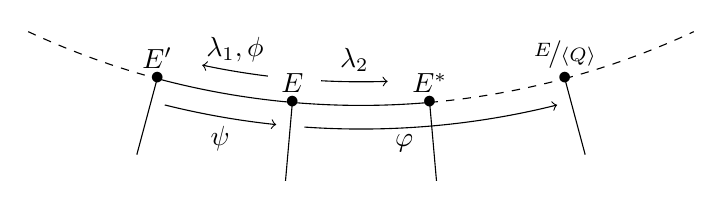
\begin{tikzpicture}[scale=1]
\coordinate (A) at (245:10);
\coordinate (B) at (255:10);
\coordinate (B') at (255:11);
\coordinate (B1) at (256:10.3);
\coordinate (C) at (265:10);
\coordinate (C') at (265:11);
\coordinate (D) at (275:10);
\coordinate (D') at (275:11);
\coordinate (E) at (285:10);
\coordinate (E') at (285:11);
\coordinate (F) at (295:10);
\coordinate (F') at (295:11);
\coordinate (G) at (305:10);
\coordinate (B2) at (258:9.7);
\coordinate (C1) at (266:10.3);
\coordinate (C2) at (267:9.7);
\coordinate (encre) at (273:10.5);
\draw (A) arc(245:255:10)[dashed];
\draw (B) arc(255:275:10);
\draw (D) arc(275:285:10)[dashed];
\draw (E) arc(285:295:10)[dashed];
\draw (B) node[above] {$E'$} node{$\bullet$};
\draw (C) node[above] {$E$} node{$\bullet$};
\draw (D) node[above] {$E^*$} node{$\bullet$};
\draw (E) node[above] {$\nicefrac{E}{\langle Q \rangle }$} node{$\bullet$};
\draw (encre) node {$\varphi$};
\draw (B)--(B');
\draw (C)--(C');
\draw (D)--(D');
\draw (E)--(E');
\draw (B1) arc(256:264:10.3) [->] node[below,midway] {$\psi$}; %flèche représentant \psi
\draw (B2) arc(258:263:9.7) [<-] node[above,midway] {$\lambda_1, \phi$}; %flèche représentant 
\draw (C2) arc(267:272:9.7) [->] node[above,midway] {$\lambda_2$}; %flèche représentant 
\draw (C1) arc(266:284:10.3) [->];% node[below,midway,fill=white] {$\varphi $};

%\draw (260:10.75) node{}
%\draw (0,0) arc (245:255:10)[dashed] node[above] {$C$} node{$\bullet$} --(0:1.5);
%\draw (0,0) arc (245:255:10)[dashed] arc (255:265:10) node[above] {$E^i$} node{$\bullet$} --(0:1.5);
%\draw (-1,0) arc (245:255:10) node[above] {$C2$} node{$\bullet$} --(90:1)[color=yellow];
%\draw (-1,0) arc (245:255:10) node[above] {$C$} node{$\bullet$} --(310:1.5)[color=red];
%\draw (0,0) arc (245:255:10)[color=white] node[above] {$C$} node{$\bullet$} arc (255:265:10) node[above] {$E^i$} node{$\bullet$} arc (265:275:10) node[above] {$E$} node{$\bullet$} arc (275:285:10) node[above] {$F$} node{$\bullet$} arc (285:295:10) node[above] {$G$} node{$\bullet$} ; 
\end{tikzpicture}
\end{center}
\caption{ Example for the case $\ell=2$ } 
\end{figure}
\begin{algorithm}
\caption{\label{alg:horizontal}Straightening $Q$ following the $\lambda_1$ direction}
\begin{algorithmic}[1]
\REQUIRE $(P, Q)$: a diagonal basis of~$E[ℓ^{h+1}]$;\\
$R$: a point of~$E[ℓ^k]$ such that
$ℓ^n R$~is horizontal of direction~$μ$ for some~$n ≤ k$.
\ENSURE $E →^{ϕ_1} E_{1} … E_{n-1} →^{ϕ_n} E_n$:
a chain of $n$ horizontal $ℓ$-isogenies of direction~$λ$;\\
$R_n$: a horizontal point of~$E_{n}[ℓ^{k}]$ of direction~$μ$.
\STATE $E_0 \gets E$; $(P_0, Q_0, R_0) \gets (P, Q, R)$
\FOR{$i = 1$ to~$n$}
\STATE $ϕ_i\gets $ isogeny with kernel ${ℓ^h P_{i-1}}$
\STATE $Q_{i} \gets ϕ(Q_{i-1})$
\STATE $P' \gets ϕ(P_{i-1})/ℓ$.
\STATE Write~$π(P') = λ P' + b Q_i$ for~$b ∈ ℤ/ℓℤ$ and
let $P_{i} \gets P' - (b/μ) Q_i$.
\STATE $R_i \gets ϕ(R_{i-1})$.
\ENDFOR
\RETURN $P,L$
\end{algorithmic}
\end{algorithm}
% \begin{prop}%<<<
\begin{prop}
Algorithm~\ref{alg:horizontal} is correct and has a complexity of
% The computation complexity of algorithm \ref{alg:diagonal} is
\begin{equation*}
\begin{array}{ll}
O\pa{\cout{M}(ℓ^k) · k · (k + \log q)}, &\text{if $ℓ = 2$;}\\
O\pa{\cout{M}(ℓ^k) · ℓ^k · k^2 · \log ℓ · \log q
  \;+\; k · \cout{F}(q, ℓ^k)}, &\text{if $ℓ ≠ 2$.}
\end{array}
\end{equation*}
\end{prop}
% Algorithm~\ref{alg:horizontal} is correct and has a computational complexity for
% \begin{enumerate}
% \item[$\ell =2$] of $O((\log(r)^2+\log(r)\log(q))M(\sqrt{r}))$ operations in $\mathbb{F}_q$,
%  \item[$\ell \neq 2$] of $O(\sqrt{r}\log(q)M(\sqrt{r})\log(r)^2 \log(\ell)^{-1}+kF(q,\ell^k))$ operations in $\mathbb{F}_q$.
%  
% \end{enumerate}
% \end{prop}%>>>
\begin{proof}
We check that at step~$i$ of the loop,
the point $ℓ^{n-i} R_i$ is horizontal with direction~$μ$,
using Proposition~\ref{prop:push-horizontal} for the induction step.
% Since $ϕ_{i+1}$ is horizontal with direction~$λ$,
% according to Proposition~\ref{prop:push-horizontal},
% $ℓ^{n-i-1} R_{i+1} = ϕ_{i+1} (ℓ^{n-i-1} R_i)$ is also horizontal
% with direction~$μ$.
The complexity analysis %of Algorithm~\ref{alg:horizontal}
is exactly the same as for Algorithm~\ref{alg:diagonal}.
\end{proof}


In practice, we shall use Algorithm~\ref{alg:horizontal}
in the case where~$R = Q_{k}$ as output from Algorithm~\ref{alg:diagonal}.
In that case, since $Q_k$~is diagonal, $ℓ^{h} Q_k$~is horizontal,
so that we may use~$n=h$.
Computing a horizontal point of order~$ℓ^k$ could be done
with Algorithm~\ref{alg:diagonal} instead,
but that would require computing in an extension
of degree up to~$ℓ^{k+h}$.

%Algorithme necessaire, surement pour enfoncer le clou...

\subsection{Proof of the algorithm}
Now that we have seen a way to determine a set of $\ell^{k}$ torsion points that generates horizontal $\ell^k$ isogenies, we have to show that this set is invariant under isogenies of degree prime to $\ell$.

\begin{prop}
For $\phi$: $E \rightarrow E'$ a $r$-isogeny  with $r \wedge \ell=1$ a prime, and $P$ a $\ell^i$ primitive torsion point, with $i>0$ such that $E \rightarrow E / \langle P \rangle $ is horizontal and $\pi(P)=\lambda_1P$. Then the isogeny  $E' \rightarrow E' / \langle \phi(P) \rangle$ is also horizontal.
\end{prop}

\begin{proof}
We just have to prove that there exists a $\ell^{h+i}$ primitive torsion point $V$ dividing $\phi(P)$ such that $\pi(V)=\lambda_1V$.
Since $P$ is a point that generates a horizontal isogeny then there exists a point $R$ of order $\ell^{h+i}$ dividing $P$. Since $\phi$ is a $r$ isogeny then $\phi$ doesn't change the order of $P$ and $R$, moreover the frobenius commutes with $\phi$ (because this one is defined on $\mathbb{F}_q$) then we have $\pi(\phi(R))=\lambda_1\phi(R)$ which proves the assertion.
\end{proof}



%%%%%%%%%%%%%%%

\section{Interpolation step}
\label{sec:interpolation}

\subsection{The structure of rational $ℓ^∞$-torsion}

\todo{tout ceci irait bien à la fin de la section 2, mais \texttt{.lock}
de Luca pour l'instant}
We again assume that $E$~is a curve with maximal endomorphism ring
and that all the points of~$E[ℓ]$ are rational,
which means that~$λ ≡ μ ≡ 1 \pmod{ℓ}$.
Let~$α = v_{ℓ} (λ - 1)$ and~$β = v_{ℓ} (μ - 1)$.
Without loss of generality, we may assume~$α ≥ β$.

\begin{prop}\label{prop:l-torsion-rationnelle}
For any integer~$n$,
the group of rational $ℓ^∞$-torsion points~$E[ℓ^∞](\F_{q^{ℓ^n}})$
is isomorphic to~$(ℤ/ℓ^{n+α} ℤ) × (ℤ/ℓ^{n + β} ℤ)$.
\end{prop}
\begin{proof}
We know that $E[ℓ^k](\F_{q^n})$ is the set of fixed points of~$π^n$.
The result follows from the diagonalization of~$π$
according to Proposition~\ref{prop:matrice-frobenius}.
\end{proof}

% Let~$(P, Q)$ be a diagonal basis of~$E[ℓ^k]$,
% and let~$R = c P + d Q$ be a a point of~$E[ℓ^k]$.
% \todo{ceci marche uniquement pour $ℓ ≠ 2$}
% We may write $c = c_0 · ℓ^γ · \exp (ℓ c_1)$
% for an unique $(ℓ-1)$-root of unity~$c_0$, integer~$γ ≤ k$,
% and~$c_1 ∈ ℤ/ℓ^{k-1} ℤ$,
% and likewise~$d = d_0 · ℓ^δ · \exp (ℓ d_1)$.
% Since~$λ ≡ 1 \pmod{ℓ}$, we also have~$λ ≡ \exp ( ℓ^{α+1} u )$
% for a unique invertible~$u ∈ ℤ/ℓ^{k-1-α}ℤ$,
% and likewise $μ = \exp ( ℓ^{β+1} v)$.
% The action of~$π^n$ on~$R$ is then given by
% $π^n (R) = c_0 · ℓ^{γ} · \exp (ℓ c_1 + n ℓ^{α+1} u) P
% + d_0 · ℓ^{δ} · \exp (d_1 + n ℓ^β v) Q$.
% We can see that two points~$R, R'$ belong to the same orbit
% if and only if, (with obvious notations):
% $c_0 = c'_0$, $d_0 = d'_0$, $γ = γ'$, $δ = δ'$,
% and $v (c_1 - c'_1) ≡ u (d_1 - d'_1) \pmod{ℓ^{k-\max (α + γ, β+δ)}}$.
% 

Let~$ξ$ be a $(ℓ-1)$-th root of unity in~$ℤ_ℓ$.
The map~$f(x, y, z) = ℓ^x· ξ^y· \exp (ℓ z)$
is a group isomorphism between~$ℤ × (ℤ/(ℓ-1) ℤ) × ℤ_ℓ$ and~$ℚ_ℓ^{×}$.
For any~$k$, it maps the triples~$(x, y, z)$
such that~$x ≤ k$, $0 ≤ y ≤ ℓ-2$, and~$0 ≤ z < ℓ^{k - x - 1}$
to $ℤ/ℓ^{k} ℤ$.

Since~$λ ≡ μ ≡ 1 \pmod{ℓ}$,
we may write~$λ = f(0, 0, λ_1)$ and~$μ = f(0, 0, μ_1)$.
Let~$λ_1 = ℓ^α u$ and~$μ_1 = ℓ^β v$ for invertible~$u, v$.
The action of~$π^n$ on~$R = c P + d Q$,
where~$c = f(γ, c_0, c_1)$ and~$d = f(δ, d_0, d_1) ∈ ℤ/ℓ^{k} ℤ$,
is given by~$π^n (R) = f(γ, c_0, c_1 + n λ_1) P + f(δ, d_0, d_1 + n μ_1) Q$.
Two points~$R, R' ∈ E[ℓ^k]$ are Galois conjugated if, with obvious notations,
$γ' = γ, δ' = δ, c_0 = c'_0, d_0 = d'_0$, and the equations
$ℓ^α n ≡ (c'_1 - c_1)/u \pmod{ℓ^{k-γ-1}}$,
$ℓ^β n ≡ (d'_1 - d_1)/v \pmod{ℓ^{k-δ-1}}$ have a solution~$n$.
The solutions of this system are given by
\begin{equation*}
\left\{\begin{array}{rcl}
c'_1 &=& c_1 + u ℓ^α x,\\
d'_1 &=& d_1 + v ℓ^β x + ℓ^{k-δ-1} y\\\end{array}\right.
\text{ for }\left\{\begin{array}{l}
0 ≤ x ≤ ℓ^{k-α-γ-1}\\
0 ≤ y < ℓ^{k-δ-1}.\end{array}\right.
% $c'_1 = c_1 + u ℓ^{α} x$ for~$0 ≤ x < ℓ^{k-α-γ-1}$
% and~$d'_1 = d_1 + v ℓ^{β} x + ℓ^{k-δ-1} y$ for~$0 ≤ y < ℓ^{k-δ-1}$.
\end{equation*}


\subsection{Interpolating a polynomial on a field extension}

In this part we solve the following problem:


\todo{\vrule height 1pt width 10cm}

In this section we consider the abscissae of points of order $\ell^k$ and generators of horizontal isogenies on the two input curves of problem \ref{prob:isogeny-problem} on a cyclic crater of volcano of $\ell$ isogeny. We want to compute an interpolation polynomial that interpolates the abscissas of thoses points. We consider the horizontal basis $(P,Q)$ of $E$ and $(P',Q')$ of $E'$ computed in the section \ref{sec:acti-frob-endm}, for this section we want to compute an interpolation polynomial $L$ that respects the mapping $P \rightarrow aP'$ and $Q \rightarrow bQ'$ with $a,b \in \left(\mathbb{Z}/\ell^k \mathbb{Z} \right)^*$ such that $L(x(cP+dQ))=x(caP+dbQ)$ for $c,d \in (\mathbb{Z}/\ell^k\mathbb{Z})^2$ with $c\wedge \ell=1$ or $d \wedge \ell =1$ and $x(P)$ which represents the abscissa of $P$. Thus the mapping will respect the fact that an horizontal basis $(P,Q)$ is sent on an other horizontal basis $(P',Q')$, respecting the direction $\lambda, \mu$ of the horizontal $\ell^k$-isogeny as a rational $r$-isogeny should do.


We state first a result on the order of the points under the action of the Frobenius.

\begin{defi}
We denote by $E(\mathbb{F}_q)[\ell^{\infty}]=\mathbb{Z}/\ell^{j+s}
\mathbb{Z} \times \mathbb{Z}/\ell^{s} \mathbb{Z}$ the structure of the rational $\ell^{\infty}$ torsion with with $j \geqslant 0$, $1 \leqslant s \leqslant \nu_\ell(q-1)$. 
\end{defi}
We consider that we work in the smaller extension field to have the entire $\ell^k$ torsion defined, then as we have supposed that $E[\ell] \subset E(\mathbb{F}_q)$ we have the following result by \ref{prop:degree-l-torsion}:

\begin{prop}
 $E(\mathbb{F}_{q^{\ell^{k-s}}})[\ell^{\infty}]=\mathbb{Z}/\ell^{k+j}
\mathbb{Z} \times \mathbb{Z}/\ell^{k} \mathbb{Z}$. 
\end{prop}

\begin{defi}
We denote by $o_{\lambda}$ and $o_{\mu}$ the multiplicative order of the
eigenvalues $\lambda , \mu \in (\mathbb{Z}/\ell^k\mathbb{Z})^2$ of the Frobenius for the
$\ell^{k}$ torsion of the elliptic curve $E$.
\newline
We denote by $o_A=\max(o_{\lambda},o_{\mu})$ and $o_B=\min(o_{\lambda},o_{\mu})$.
We will suppose without loss of generality that $P$ (resp. $Q$) has an eigenvalue $\lambda$ (resp. $\mu$) of order $o_A$ (resp. $o_B$) for the Frobenius, with $(P,Q)$ the horizontal basis computed in section \ref{sec:acti-frob-endm}.
\end{defi}

\begin{prop}
$o_A=\max(o_{\lambda},o_{\mu}) = \ell^{k-s}$ and $o_B=\min(o_{\lambda},o_{\mu}) = \ell^{k-j-s}$
\end{prop}

\begin{proof}
%By proposition \ref{structelevation} we have $E[\ell^{k+s}] \subset E(\mathbb{F}_{q^{\ell^k}})$ and $E[\ell^{k+s}] \not \subset E(\mathbb{F}_{q^{\ell^{k-1}}})$ and $E(\mathbb{F}_{q^{\ell^{k-j}}})[\ell^{\infty}]=  \mathbb{Z}/\ell^{s+k}\mathbb{Z} \times \mathbb{Z}/\ell^{s+k-j}\mathbb{Z}$ and $E(\mathbb{F}_{q^{\ell^{k-j-1}}})[\ell^{\infty}]=  \mathbb{Z}/\ell^{s+k-1}\mathbb{Z} \times \mathbb{Z}/\ell^{s+k-j-1}\mathbb{Z} $
%By structure of the $E(\mathbb{F}_{q})[\ell^{\infty}]$ the smallest field where all the entire $\ell^k$ torsion is defined is $\mathbb{F}_{q^{\ell^{k-s}}}$ thus we have point of $\ell^k$ torsion defined only in $\mathbb{F}_{q^{\ell^{k-s}}}$ which gave us  $o_A=\max(o_{\lambda},o_{\mu}) = \ell^{k-s}$. For $o_B=\min(o_{\lambda},o_{\mu}) = \ell^{k-j-s}$ we have to notice that field where $\ell^k$ torsion 

%Let consider a point $P$ of order $\ell^{k+s}$ associated to $\max(o_{\lambda_1},o_{\lambda_2})$, then we will have by definition of $o_{\lambda_1}$ and $o_{\lambda_2}$: $\pi(P)^{\max(o_{\lambda_1},o_{\lambda_2})}=P$, as $P$ is a point of order $2^{k+h}$ by the proposition \ref{structelevation} he is defined at least in $\mathbb{F}_{q^{\ell^{k-j}}}$ and at most in $\mathbb{F}_{q^{\ell^k}}$ thus we have the results.
%\todo{Fix this; not understandable, not a proof.}
 Let $P$ be a point of order $\ell^k$, by the structure of $E(\mathbb{F}_q)[\ell^{\infty}]$ and by \ref{prop:degree-l-torsion} we have points defined in $\mathbb{F}_{q^{\ell^{k-j-s}}}$ , for those points we will have $\pi^{\ell^{k-j-s}}(P)=P$ and $\pi^{\ell^{k-j-s-1}}(P) \neq P$ otherwise they would be defined in $\mathbb{F}_{q^{\ell^{k-j-s-1}}}$ which would contradict the structure of $E[\ell^{\infty}]$. We have points $P$ of order $\ell^k$ only defined in $\mathbb{F}_{q^{\ell^{k-s}}}$, for them we have $\pi^{\ell^{k-s}}(P)=P$ and $\pi^{\ell^{k-s-1}}(P) \neq P$ otherwise if would contradict the structure of $E(\mathbb{F}_q)[\ell^{\infty}]$
\end{proof}

%For the rest of this section we will consider that $s=1$ to be in the worst case.\todo{What does this mean? It means that the worst case is when we have to work in high extension field to have the $\ell^k$ torsion defined}

Since the isogeny we want to compute is rational and we work with
points that are defined in extensions of the base field, we will work
with points that are in different orbits under the action of the
Frobenius. As the size of the orbits are not always the same, we will
have to consider the different possible orders and combine them
efficiently.

\begin{defi}
  For $i$ in $\{0, \dots,\nu_{\ell}(o_A)-\nu_{\ell}(o_B)=j\}$, we denote by $o_i$
  the integer $o_i =\frac{o_A}{\ell^i} \in \{o_B,\dots,o_A\}$.
\end{defi}

%\begin{defi}
 % We define $o_A=\max(o_{\lambda_1},o_{\lambda_2})$ and
 % $o_B=\min(o_{\lambda_1},o_{\lambda_2})$, where for $i$ in $\{1,2\}$,
 % $o_{\lambda_i}$ is the order of the eigenvalue $\lambda_i$ in
 % $\mathbb{Z}/\ell^k\mathbb{Z}$. In particular, $o_A=O(\ell^k)$.
%\end{defi}

%% \begin{defi}
%% We define the cost of computing the Frobenius on a finite field of size $q^{n}$ with the complexity expressed in terms of operations on $\mathbb{F}_q$ by the following function: $F(q,n)$.
%% \end{defi}


\begin{defi}
For $i$ in $\{0,\dots j\}$ we define the sets
$I_i$ of points of order $\ell^k$ and of orbits of length $o_i$ for the Frobenius as follows:
\newline
For $0 < i < \nu_{\ell}(o_A)-\nu_{\ell}(o_B)$:
$I_i=\{ \ell^i c P + d Q, (c,d) \in \left( \mathbb{Z}/ \ell^k \mathbb{Z}^{*} \right)^2 \} $ \todo{Nom de variable moche ouvert à suggestion}
\newline
$I_j=\{ \ell^j c P + d Q, (c,d) \in \left( \mathbb{Z}/ \ell^k \mathbb{Z} \right)^2, d \wedge \ell =1 \} $
\newline
$I_0=\{ c P + d Q, (c,d) \in \left( \mathbb{Z}/ \ell^k \mathbb{Z} \right)^2, c \wedge \ell =1 \}$
\end{defi}

%For $i$ in $\{0,\dots \nu_{\ell}(o_A)-\nu_{\ell}(o_B)\}$ we define the polynomials
%$T_i$ and $L_i$ as follows:
%\begin{itemize}
%\item $T_i= \prod_{R \in I_i} (x-x(R))$
%\item $L_i$ is the Lagrange interpolation polynomial that send: $x(\ell^i c P + d Q)$ on $x(\ell^i c aP' + d b Q')$ for every  $ \ell^i c P + d Q  \in I_i $ and $a,b \in \left( \mathbb{Z}/ \ell^k \mathbb{Z} \right)^{*}$ the parameters for the interpolation mapping.
%\end{itemize}
We won't work directly with $I_i$ we consider the action of the Frobenius and thus we will work with the following sets.
\newline
\begin{defi}
For $i$ in $\{0,j\}$ we define the sets
$\mathcal{I}_i$ of points of order $\ell^k$ and representative of orbits of length $o_i$ for the Frobenius as follows:
\newline
For $0 \leqslant i \leqslant j $:
$\mathcal{I}_i=\{ R \in I_i, \pi^t(R) \notin \mathcal{I}_i, t \in \{0.. o_i\} \} $ 
\end{defi}
The sets $\mathcal{I}_i$ are not uniquely defined. In practice we compute the index of these points $R \in \mathcal{I}_i$ in the basis $(P,Q)$ and then we take the corresponding points. The choice of representants of orbits is not important since we will consider then the action of the Frobenius and thus all the points of $I_i$.
\newline
We define for $i$ in $\{0,\dots j\}$ the polynomials
$\mathcal{T}_i$ and $\mathcal{L}_i$ as follows:
\begin{itemize}
\item $\mathcal{T}_i= \prod_{R \in \mathcal{I}_i} (x-x(R))$
\item $\mathcal{L}_i$ is the Lagrange interpolation polynomial that send: $x(\ell^i c P + d Q)$ on $x(\ell^i c aP' + d b Q')$ for every  $ \ell^i c P + d Q  \in \mathcal{I}_i$ and $a,b \in \left( \mathbb{Z}/ \ell^k \mathbb{Z} \right)^{*}$ the parameters for the interpolation mapping.
\end{itemize}


\begin{lem}
  For $i$ in $\{0, \dots,j\}$, the
  polynomials $\mathcal{T}_i$ and $\mathcal{I}_i$ are defined over
  $\mathbb{F}_{q^{o_i}}$ and of degree $d_i$. $d_i=\ell^{k-1+s}$ for $i$ in $\{1, \dots,\nu_{\ell}(o_A)-\nu_{\ell}(o_B)\}$ and $d_0=\ell^{k-2+s}$.
\end{lem}

\begin{proof}
  Since $\mathcal{T}_i$ is a polynomial defined with abscissae of
  points of order $\ell^k$  which are representative of orbits of order $o_i$ under the Frobenius action  we then have $\mathcal{T}_i \in \mathbb{F}_{q^{o_i}}[x]$. The fact that we take representants of different orbits permtis us to conclude. We can apply the same reasoning for $\mathcal{I}_i$.\todo{Not clear, I don't understand
    (especially the ``because \dots'').} \todo{What about $I_j$?}
    \newline
For $0 < i < j$ the set $I_i$: is of size $\ell^{2k-2-i}$. Then to obtain $\mathcal{I}_i$ we take each abscissa of representant of the orbits of order $o_i$, which gave us the size $\ell^{k-2+s}$
\newline
The set $I_0$ is of size $\ell^{2k-1}$. Then we take each abscissa of representant of the orbits of order $o_A$, which gave us the size $\ell^{k-1+s}$ for $\mathcal{I}_0$
\newline
The set $I_j$ is of size $\ell^{2k-1} \frac{o_B}{o_A}$. Then we take each abscissa of representant of the orbits of order $o_B$, which gave us the size $\ell^{k-1+s}$   for $\mathcal{I}_j$
\end{proof}

%Using the action of the Frobenius, we will then get the vanishing
%(resp. interpolation) polynomials defined on all the orbit \todo{which
%  orbit?}. To avoid any redundant Frobenius action we have to add a
%different order after a Frobenius action. \todo{I don't understand}
\begin{defi}
We denote by $\sigma$ the action of the frobenius on coefficients of a polynomial.
\end{defi}

Our aim is to deduce from the different polynomials $\mathcal{T}_i,
\mathcal{I}_i$ the polynomials
$$T=\prod_{i=0}^{\nu_{\ell}(o_A)-\nu_{\ell}(o_B)}\prod_{t=1}^{o_i}\sigma^{t}(\mathcal{T}_i)$$ 
and
$$I= CRT(\sigma^{t}(\mathcal{L}_j) \bmod \sigma^{t}(\mathcal{T}_j), i\in \{ 0,.., \nu_{\ell}(o_A)-\nu_{\ell}(o_B) \}  t \in \{ 1,..,o_i \} )$$
with $CRT$ the Chinese Remainder Theorem.

\begin{prop}
$T ,L $ are defined over $\mathbb{F}_q$ and of degree $3\ell^{2k-2}$. $T$ (resp. $L$) vanishes (resp. interpolates) on all the abscissas of point of order $\ell^k$ of the curve $E$ (resp. of the curve $E$ on $E'$) according to the mapping coefficients $(a,b) \in \left( \mathbb{Z}/ \ell^k \mathbb{Z} ^* \right)^2$.  
\end{prop}

\begin{proof}
$\sigma(T)=\prod_{i=0}^{\nu_{\ell}(o_A)-\nu_{\ell}(o_B)}\prod_{t=2}^{o_i+1}\sigma^{t}(\mathcal{T}_i)$
since $\mathcal{T}_i \in \mathbb{F}_{q^{\ell^{o_i}}}$ then $\sigma^{o_i+1}(T)=\sigma(\sigma^{o_i}(T))=\sigma(T)$, thus we have $\sigma(T)=T$. We can apply the same reasoning for $I$.
\newline
Every point $P$ of order $\ell^k$ has by definition an order $o_B \leqslant o \leqslant o_A$, then either the abscissa of $P$ is a root of $\mathcal{T}_i$ either $P$ belongs to the orbit of a point which abscissa is a root of $\mathcal{T}_i$ since with the successive actions of the Frobenius we get all the entire orbit we will get the abscissa of $P$. The same demonstration can be done for $I$. We get the degree of $I$ and $T$ by counting the number of points of degree $\ell^k$ knowing that $E[\ell^{k}] \subset \mathbb{F}_{q^{\ell^k}}$.
\newline 
Let $R=(cP+dQ)$ a point of order $\ell^k$, such that $R$ is a root of a $\mathcal{T}_i$ for $i \in \{ 0 ..j \} $ then  for every $t \in \{0..o_i \}$ by construction of $L$ we have  $L = \sigma^{t}(\mathcal{L}_i)  \bmod  \sigma^{t}(\mathcal{T}_i)$ thus  $=L(x(c\lambda^tP+d\mu^tQ))=L(\pi^t(x(R)))=\pi^t(L(x(R)))=\pi^t(x(caP'+dbQ'))=x(ca\lambda^tP'+db\mu^tQ')$. Since every point of order $\ell^k$ belongs to the orbit of one of the $\mathcal{T}_j$ we have $L$ that interpolates conformly with the mapping coefficients $a$ and $b$.
\end{proof}

\todo{Prove that these polynomials satisfy the requirements of the 
main algorithm. For the moment, we have {\bf no idea} of what interpolates
what, and how the conditions given at step 2 of the Algo of 6.1 
are necessarily satisfied by the polynomial $A$ we compute here.}



%% using the combined actions of the Frobenius with Chinese Remainder
%% techniques.

We won't compute $T$ and $I$ directly as in their definition. We will compute them in a way at each step $i$ we consider all the polynomials defined in $\mathbb{F}_{q^{\frac{o_A}{\ell^i}}}$ and use a combined action of the Frobenius and chinese remainder techniques to have a result defined in $\mathbb{F}_{q^{\frac{o_A}{\ell^{i+1}}}}$
  
%We start by taking into account the greatest orbit with the
%polynomials $\mathcal{I}_0$, $\mathcal{T}_0 \in
%\mathbb{F}_{q^{o_A}}[x]$, which has order $o_A$ for the Frobenius
%action; we obtain polynomials $R$ and $S$ $\in
%\mathbb{F}_{q^{\frac{o_A}{\ell}}}[x]$ with a combined action of the
%Frobenius with Chinese remainder techniques on the polynomials
%$\mathcal{I}_0$, $\mathcal{T}_0$. Then with $R$ and $S$ of order
%$\frac{o_A}{\ell}$ for the Frobenius action we take into account the
%polynomials of same order for the Frobenius action $\mathcal{I}_1$,
%$\mathcal{T}_1 \in \mathbb{F}_{q^{\frac{o_A}{\ell}}}[x]$ and we use
%again a combined action of the Frobenius with Chinese remainder
%techniques on these polynomials to obtain new polynomials $R$ and $S$
%$\in \mathbb{F}_{q^{\frac{o_A}{\ell^2}}}[x]$. We repeat those
%operations until we get polynomials $R$ and $S$ $\in
%\mathbb{F}_{q^{\frac{o_B}{2}}}[x]$. From this point we only use a
%combined action of the Frobenius with Chinese remainder techniques
%until we get $A$ and $T \in \mathbb{F}_q[x]$.

%%  and
%% then we make act the frobenius on this polynomial (both
%% $\mathcal{T}_A$ and $\mathcal{A}_A$) then with the CRT we have a new
%% interpolation polynomial that take into account the frobenius
%% action. We take then into account the next greater order together with
%% the previous polynomial obtained and we repeat this until we get to
%% the order $o_B$. After this we only make act the Frobenius until we
%% have every element of the orbits.

%% At each step we obtain a new interpolation polynomial $A_j$ from the CRT of two other polynomials, we do some pre-computation to fasten the next CRT computation since the modulus do not change at each interpolation try of the algorithm.

\begin{algorithm}
\caption{\label{computingT2ir} Computing $I,T \in \mathbb{F}_q[x]$} 
\begin{algorithmic}[5]
\REQUIRE All the polynomials $\mathcal{T}_j, \mathcal{I}_j \in \mathbb{F}_{q^{o_j}}$ for $j \in [0, \nu_{\ell}(o_A)-\nu_{\ell}(o_B)]$. 
\ENSURE $T=\prod_{i=0}^{\nu_{\ell}(o_A)-\nu_{\ell}(o_B)}\prod_{t=0}^{o_i}\sigma^{t}(\mathcal{T}_i)$ $I= CRT(\sigma^{t}(\mathcal{I}_j) \bmod \sigma^{t}(\mathcal{T}_j), i\in \{ 0,.., \nu_{\ell}(o_A)-\nu_{\ell}(o_B) \}  ,t \in \{ O,..,o_i \} ) \in \mathbb{F}_q[x]$
%\STATE \textit{Compute} $\mathcal{A}_A$ %\STATE $\left( \sigma^{o_A/2}(\mathcal{T}_A),\sigma^{o_A/2}(\mathcal{A}_A) \right) \gets \left( \mathcal{T}_A,\mathcal{A}_A \right) \in \mathbb{F}_q^{o_A}[x]$
\STATE $\left( R,T \right) \in \mathbb{F}_{q^{o_A/\ell}}[x] \gets CRT \left( \sigma^{o_A/\ell}(\mathcal{I}_A) \bmod  \sigma^{o_A/\ell}(\mathcal{T}_A),\mathcal{I}_A \bmod \mathcal{T}_A \right)$
\FOR{$r=1$ to $\nu_\ell(\frac{o_{A}}{o_{B}})$}%\STATE $\left( R_2=\sigma(R)^{o_A/2^{1+r}} T_2=\sigma(T)^{o_A/2^{1+r}} \right) \gets \left( R,T \right) \in \mathbb{F}_{q^{o_A/(2^r)}}$
\STATE $\left( R , T \right) \in \mathbb{F}_{q^{o_A/(\ell^{r+1})}}[x] \gets CRT \left( \sigma^{o_A/\ell^{1+r}}(R) \bmod \sigma^{o_A/\ell^{1+r}}(T), R \bmod T \right) $ 
%\STATE \textit{Compute} $\mathcal{A}_r$%\STATE $\left( \sigma^{o_A/2^{1+r}}(\mathcal{T}_r), \sigma^{o_A/2^{1+r}}(\mathcal{A}_r) \right) \gets \left( \mathcal{T}_r , \mathcal{A}_r \right) \in \mathbb{F}_{q^{o_A/(2^r)}}$  
\STATE $\left( B,T_B \right)\in \mathbb{F}_{q^{o_A/\ell^{(r+1)}}}[x]  \gets CRT \left( \sigma^{o_A/\ell^{1+r}}(\mathcal{I}_r) \bmod \sigma^{o_A/\ell^{1+r}} (\mathcal{T}_r),\mathcal{I}_r \bmod \mathcal{T}_r, \right)$ 
\STATE $\left( I,T \right) \gets CRT \left(B \bmod T_B, R \bmod T \right) $
\ENDFOR
\FOR{$r=1$ to $\nu_\ell(o_B)-1$}%\STATE $\left( R_2=\sigma(R)^{o_B/2^{1+r}}, T2=\sigma(T)^{o_B/2^{1+r}} \right) \gets \left( R,T \right) \in \mathbb{F}_{q^{o_B/(2^r)}} $
\STATE $\left( I , T \right)\in \mathbb{F}_{q^{o_B/(\ell^{(r+1)}}} \gets CRT \left( I \bmod T ,\sigma^{o_B/\ell^{1+r}}(R) \bmod \sigma^{o_B/\ell^{1+r}}(T) \right)$
\ENDFOR
\RETURN $A,T$
\end{algorithmic}
\end{algorithm}

Before giving the complexity analysis of this algorithm, we describe
the cost of some basic operations used in it. The first result is
Lemma~2.2 in~\cite{vzgathen+shoup92}.  \todo{Is it wise to use $k$
  here? Isn't $k$ already fixed?}
\todo{we don't need this before, by the way?}

\begin{lem}\label{lemma:complexity_pol_mul} Let $t$ be an integer
  The cost of multiplying two polynomials of degree $n$ in
  $\mathbb{F}_{q^{\ell^t}}[x] $ is $O(\mathsf{M}(\ell^tn))$ operations in
  $\mathbb{F}_q$.
\end{lem}

\begin{prop}Let $t$ be an integer,
the cost of the Chinese Remainder Theorem for two polynomials of
degree $n$ of $\mathbb{F}_{q^{\ell^t}}[x] $ is of
$O(\mathsf{M}(\ell^tn)\log(n))$ operations in $\mathbb{F}_q$.
\end{prop}

\begin{proof}
We obtain this result by adapting the proof of the Theorem $11.5$ of \cite{vzGG}.
\end{proof}

Since we can do some pre computation for the C.R.T. we have his cost that changes. 

\begin{prop}Let $t$ be an integer,
for $A, T_A,B, T_B,U,V \in \mathbb{F}_{q^{t}}[x]$ of degree inferior to $n$ such that $U=0 \bmod T_A$, $U=1 \bmod T_B$ $V=1 \bmod T_A$, $V=0 \bmod T_B$ . The cost of $CRTs(A \bmod T_A,B\bmod T_B)$ is of $M(nt)$ on $\mathbb{F}_q$.
\end{prop}

\begin{prop}
For $ o_{B} \leqslant o_i \leqslant o_{A}$ we have $\mathcal{T}_j$ and $\mathcal{L}_i$ of degree $d: \ell^{k-2+s}  \leqslant d \leqslant \ell^{k-1+s}$ in $\mathbb{F}_{q^{o_i}}$. 
\newline
For $\ell=2$ the cost of computing the different $\mathcal{T}_i,\mathcal{L}_j$ is of $O(\mathsf{M}(2^{k+s})\log(2^{k+s}))$ operations on $\mathbb{F}_{q^{o_j}}$, thus $O(\mathsf{M}(\frac{2^{2k}}{2^j})\log(2^{k}))$ in $\mathbb{F}_q$.
\newline 
For $\ell \neq 2$ the cost of computing the different $\mathcal{T}_i,\mathcal{L}_j$ is of $O(\mathsf{M}(\ell^{k+s})\log(\ell^{k+s}))$ operations on $\mathbb{F}_{q^{o_j}}$, thus $O(\mathsf{M}(\ell^{k+s})\mathsf{M}(\ell^{o_j}) \log(\ell^{o_j})\log(\ell^{k+s}))$ in $\mathbb{F}_q$. %peut etre preciser ici que je me sers du papier de tours \ell adique de Luca Jawad et Eric
\end{prop}

\begin{proof}\todo{Regarder si cette preuve ne devient pas inutile avec la section 2}
When $\ell=2$ by \cite{DoSc12} the cost of an inversion of elements in $\mathbb{F}_{q^{2^k}}$ of $\mathsf{M}(2^k)$ so we got the result. When $\ell \neq 2$ by \cite{DeDoSc13} the cost of an inversion of elements in $\mathbb{F}_{q^{\ell^k}}$ of $\mathsf{M}(\ell^k)\log(\ell^k)$ so we got the result.
\end{proof}


We remind that we have two different cost for the C.R.T. one for the pre computation, one for the next occurrences, thus we have two complexity analysis for algorithm \ref{computingT2ir}.

\begin{prop} %cout total de l'algorithme
The computational cost of algorithm \ref{computingT2ir} with the knowledge of all $\mathcal{T}_j$ and $\mathcal{A}_j$ with $  o_B \leqslant o_j \leqslant o_A$  is of:
$O(\mathsf{M}(2^{2k})k^2+ 2^{2k}\log(q))
$
operations in $\mathbb{F}_q$ for the first occurrence for $\ell=2$. For the next occurrences we have a complexity of:
$
O(\mathsf{M}(2^{2k})k+2^{2k}\log(q))
$
operations in $\mathbb{F}_q$
\newline For $\ell \neq 2$ the complexity is of $
O(M(\ell^{2k})k^2+ \ell^{2k}F(q,\ell^k))
$
operations in $\mathbb{F}_q$ for the first occurrence. For the next occurrences we have a complexity of:
$
O(\mathsf{M}(\ell^{2k})k+\ell^{2k}F(q,\ell^k))
$
operations in $\mathbb{F}_q$

\end{prop}

\begin{proof}
For the first occurrence of algorithm \ref{computingT2ir} at each step we compute a C.R.T. on polynomials of order $O(\frac{\ell^{2k}}{o_j})$ on $\mathbb{F}_{q^{o_j}}$ with a complexity of $O(\mathsf{M}(\ell^{2k})\log(\frac{\ell^{2k}}{o_j}))$ in $\mathbb{F}_q$. At each step we compute a Frobenius which cost us $O(2^{2k}+\frac{2^{2k}}{o_A}\log(q))$ operations in $\mathbb{F}_q$ for $\ell=2$ since we have a cost for the Frobenius of $O(2^j+\log(q))$ in $\mathbb{F}_{q}$ for elements in $\mathbb{F}_{q^{o_{j}}}$ according to \cite{DoSc12} multiplying this by the degree of the polynomials considered gave us the result. For $\ell \neq 2$ the Frobenius cost us at each step $O(\frac{\ell^{2k}}{o_A}F(q,\ell^k))$ operations in $\mathbb{F}_q$.
 For the next occurrence at each step we compute a simplified C.R.T. on polynomials of order $O(\frac{\ell^{2k}}{o_j})$ on $\mathbb{F}_q{o_j}$ with a complexity of $O(M(\ell^{2k}))$ in $\mathbb{F}_q$.
Since we have to repeat those steps up to $k$ times we got the result.
\end{proof}


The computational cost of the interpolation step is of $O(rM(r)\log(r))$ since the cost of the precomputations are of $O(\mathsf{M}(r)\log(r)^2)$ and we got to repeat the interpolation try $O(r)$ times until we find the good interpolation.


\section{Complete algorithm}
\label{sec:complete-algorithm}
\subsection{Shape of the volcano and path to the crater}
	\label{sub:shape-volcano}
\todo{Eventually explicit the complexity of computing a shape of the volcano i.e. $\mathcal{F}(\ell)$}
  For the input curves we have to determine if the curves are on a volcano with cyclic crater. 
  
  For $\ell \neq 2$ we have to locate a curve on the crater and then look for  the length of $(\ell+1)$ descending paths on the volcano as described in \cite{volcano}. If there is two paths of length greater than the others then the crater is cyclic, if not the crater is not cyclic. This is done in a complexity of $O( ( \frac{\log(q)}{\log(\ell})^2 \mathcal{F}(\ell) )$, with $h=O(( \frac{\log(q)}{\log(\ell}))$ the height of the volcano (not known a priori) and $\mathcal{F}(\ell)$ the cost of computing three roots of a $\ell$ modular polynomial of $O(\ell^2+M(\ell)\log(q))$. We can also mention methods used in \cite{IonicaJ10} which are done in a complexity of $O(h(\ell^3+\ell \mathsf{M}(\ell) \log(q)))=O(( \frac{\log(q)}{\log(\ell})(\ell^3+\ell \mathsf{M}(\ell) \log(q)))$ and take advantage of the structure of the $\ell$ torsion when it is linked with the level in volcano with pairings that determine ascending or horizontal $\ell$-isogenies. %when the curve is not located over a stability level.
\newline 
For $\ell=2$ we can use methods like in \cite{MiretMRV05}. The height and the shape of the volcano can be computed with a complexity of $O(\log^6(q))$ which computes an ascending path and can determine the shape of the crater by taking advantage of the torsion structure when it is linked with the level in volcano otherwise it uses methods similar to \cite{volcano}.
 %c est exactement ce qui est fait dans ce papier...
  
 \subsection{Curves which are on the cyclic crater}
  The previous sections \ref{sec:acti-frob-endm}, \ref{sec:interpolation} describe steps of the algorithm for curves located on the crater of cyclic volcano (Elkies) thus for this subsection we consider two input curves at the problem \ref{prob:isogeny-problem} in this situation. As like the Couveignes' algorithm we proceed in 3 steps to solve problem \ref{prob:isogeny-problem}:
 \begin{enumerate}
\item Compute horizontal basis $P,Q$ and $P',Q'$ of
  $E[\ell^k]$ and $E'[\ell^k]$ respectively, for $3\ell^{2k-2} > 4r$ \todo{preciser cette borne} ;
\item\label{alg:modif-couveignes:interp} Compute the interpolation
  polynomial $\mathcal{A}$ \todo{(verify that notation is consistent
    with Sec.5)} sending $x(P)$ to $x(P')$ and $x(Q)$ to $x(Q')$, and the abscissas of
  their scalar multiples accordingly;
\item\label{alg:modif-couveignes:rational} Deduce a rational fraction
  congruent to $\mathcal{A}$ modulo $T$, and verify that it
  defines an isogeny of degree $r$. If it does, return it, otherwise
  replace $P',Q'$ with an other horizontal basis of $E'[\ell^k]$ and go back to
  Step~\ref{alg:orig-couveignes:interp}.
\end{enumerate} 

\begin{prop}
The complexity of solving problem \ref{prob:isogeny-problem} for two elliptic curves located on a cyclic crater of volcano of $\ell$ isogeny is for $\ell=2$ of $O(rM(r)\log(r))$ in $\mathbb{F}_q$ and for $\ell \neq 2$ of $O(rM(r)\log(r)+r^2F(q,\ell^k))$ in $\mathbb{F}_q$.
\end{prop}

\begin{proof}
The cost of computing horizontal basis is for $\ell=2$ of $O((\log(r)^2+\log(r)\log(q))M(\sqrt{r}))$ in $\mathbb{F}_q$, for $\ell \neq 2$ it is of $O(\sqrt{r}\log(q)M(\sqrt{r})\log(r)^2 \log(\ell)^{-1}+kF(q,\ell^k))$ in $\mathbb{F}_q$.
The cost of computing an interpolation polynomial is for $\ell=2$ of $O(M(r)\log(r))$, for $\ell \neq 2$ it is of $O(M(r)\log(r)+rF(q,\ell^k))$ . The rational reconstruction is done in $O(M(r)\log(r))$ operations in $\mathbb{F}_q$. In average we have to repeat this step $O(\ell^{2k})=O(r)$ times. 
Thus we have a total complexity for $\ell=2$ of  $O(rM(r)\log(r))$ in $\mathbb{F}_q$ and for $\ell \neq 2$ of $O(rM(r)\log(r)+r^2F(q,\ell^k))$ in $\mathbb{F}_q$.
\end{proof}
  
  \subsection{Curves which are not on the cyclic crater}

If the two input curves~$E$, $E'$ of our algorithm
belong to cyclic $ℓ$-isogenies volcanos but not to their crater,
then by Proposition~\ref{prop:isogenie-premiere},
their depth below the craters is the same.
Using the methods of~\ref{sub:shape-volcano},
we can compute the shortest path of $ℓ$-isogenies~$α: E → E_{\max}$,
$α': E' → E'_{\max}$ linking the curves~$E, E'$ to the craters.
By Proposition~\ref{prop:isogenie-premiere} (iii),
the curves~$E_{\max}$ and~$E'_{\max}$ are again $r$-isogenous;
we can use our algorithm to compute such an isogeny~$ψ_{\max}$.
Then $ψ = (α')^{-1} ∘ ψ_{\max} ∘ α$ is the required $r$-isogeny.

  \subsection{Curves which are not on a cyclic volcano}
  %We take another \ell and we cross our fingers.
  For curves which are not on an Elkies volcano we change $\ell$ and we take another prime number and we test if this new one is an Elkies prime. For every prime we have a probability of $\frac{1}{2}$ to be an Elkies prime. 


%%%%%%%%%%%%%%%

\section{Experimental results}
\label{sec:implem}

\todo{Describe implementation and show benchmarks. Possibly compare
  with Lercier-Sirvent (Luca has an implementation somewhere).}

\begin{acknowledgements}
  We thank many people.
\end{acknowledgements}

\bibliographystyle{alpha}
\bibliography{refs}


\appendix
\section{Isogenies and the Tate module}
We recall here a few results about $ℓ^n$-isogenies
and the $ℓ$-adic Tate module.

For any integer~$n$, there exists a canonical bijection~\cite[II.1.1]{SL2}
between points of order~$ℓ^n$ of~$E$
and lattices of index~$ℓ^n$ in the $ℤ_ℓ$-module~$T_ℓ(E)$:
it maps a point~$P$ to the lattice~$Λ_P = P + ℓ^n T_ℓ (E)$.
If a basis~$(R, S)$ of~$E[ℓ^n]$ is fixed and~$P = a R + b S$,
then the lattice~$Λ_P$ is generated by the columns of the matrix
$M_P = \smat{ℓ^{n-m} & a/b' \\ 0 & ℓ^m}$, where $b = ℓ^m b'$ with~$ℓ ∤ b'$.
We check that $M_P$ has determinant~$ℓ^n$.

The lattice $Λ_P$~is exactly the preimage
by the isogeny~$ϕ_P: E → E'$ of the lattice~$ℓ^n T_ℓ(E')$.
This implies that there exist bases of~$T_ℓ(E), T_ℓ(E')$
in which $Φ_P$ has the matrix~$ℓ^n M_P^{-1}$.
Therefore, the matrix of~$π' = π|T_ℓ(E)$
is conjugated, over~$ℤ_ℓ$, to $M_P^{-1} . π · M_P$.

\end{document}
%  LocalWords:  isogeny morphisms Isogenies isogenies isogenous
%  LocalWords:  cardinality bijection Couveignes automorphism

% vim: ts=2:
%  LocalWords:  Frobenius endomorphism
